\subsection{DRSSTC}
\label{DRSSTC}

\begin{figure}
    \centering
    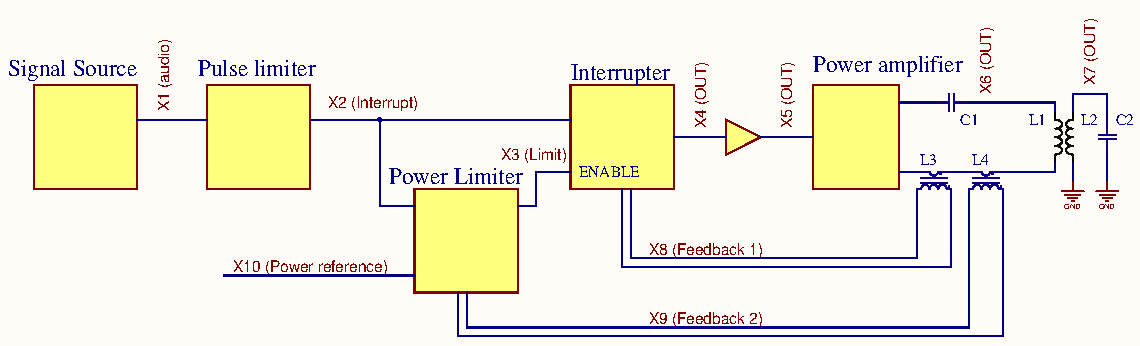
\includegraphics[width=\textwidth]{img/FunksjonsBlokkskjema.pdf}
    \caption{Block diagram}
    \label{fig:func_block}
\end{figure}

DRSSTC is an acronym for Dual Resonant Solid State Tesla Coil. Dual resonant means that we have two resonant circuits inductively coupled, and tuned to the same resonance frequency. Solid state means that we drive these resonant circuits actively with transistors. The origins of the DRSSTC is not well documented but it is commonly accepted that it was conceived on "The tesla coil mailing list" \citep{pupman}.

The signal pathway consists of a signal source, pulse shaper, power limiter, interrupter, amplifier, power amplifier.
The signal source provides the signal to be output on the coil, often the signal source is a musical recording.
The input signal should be monophonic, arpeggio\footnote{The sounding of the notes of a chord in rapid succession instead of simultaneously.} may be used. The input signal may be two level.

First the input signal $X1$ goes into the pulse shaper, which transforms the signal to two level \todo{figur}, limits on-time of each pulse, and enforces a minimum time between pulses (as explained in \cref{timing_diagrams}). Then the signal X2 is connected to the interrupter which on a positive flank outputs a positive flank X4, which is amplified $X5$ and $X6$ and sent into the resonant circuit (C1, and L1). This triggers the step response of the resonant circuit. Then a positive feedback loop $X8$ drives $X4$ at the resonant frequency of the resonant circuit (the resonant frequency is in the order $f_0 = 100k$Hz). This is achieved by inverting the output when the current through C1 and L1 passes through zero (as measured through L3). This continues until either the input pulse $X2$ goes low or the limit signal from the limiter X3 goes low.
The limiter also measures the current flowing through C1 and L1, but this signal X9 is rectified and fed through a low pass filter before being compared to a preset level X10. This comparison measures the power dissipated in the resonant circuit. If the power exceeds the preset level the enable signal X3 is set low until the next rising edge of the input signal X2.\todo{Update figure with X10} X10 is set by a multi turn potentiometer.

The resonant circuitry consists of C1, L1, C2 and L2, where L2 is magnetically coupled with L1 with a degree of approximately 0.2. C1 is a bank of capacitors with high voltage and current rating and low equivalent series resistance (ESR). L1 is an inductor with high cross section area and few turns (in the magnitude of 5 turns). L2 is an inductor with low cross section area and a high number of turns (in the magnitude of 4000 turns). C2 consists of a sphere or toroid for one plate, and the grounded (safety ground) surroundings. Ground is connected through the safety ground in the electrical socket used to power the DRSSTC.

L3 and L4 are current sensing transformers.

\subsubsection{Timing diagrams}
\label{timing_diagrams}
\cref{fig:drsstc1} to \cref{fig:drsstc6} shows different examples of input pulses, and corresponding output pulses. Note that the timings and frequencies are not to scale, only relative timings.

\Cref{fig:drsstc1} shows a single pulse on the input signal $X1$, here we see $X2$ is limited to a certain width. We also see that $X4$ and $X8$ goes high when $X2$ goes high, oscillates at the resonance frequency of the resonance circuit, and goes low when $X2$ goes low. \Cref{fig:drsstc2} shows the same principle, only with a longer pulse on $X1$.

\Cref{fig:drsstc3} shows the same input signal as \cref{fig:drsstc2} but with a different setting of the on-time on the pulse limiter (allowing longer on-time).

\Cref{fig:drsstc4} to \cref{fig:drsstc6} shows multiple pulses on $X1$ and corresponding signals on $X2$. With on-time set to 2 units and minimum time between pulses set to 12 units.

\begin{figure}[!ht]
    \centering
    \begin{tikztimingtable}
        X1 & 5L 20H 18L\\
        X2 & 5L 10H 28L\\
        X3 & 43H \\
        X4 & 5L 10{1C} 28L\\
        X8 & 5L 10{1C} 28L\\
    \end{tikztimingtable}
    \caption{One pulse on X1}
    \label{fig:drsstc1}
\end{figure}{}

\begin{figure}[!ht]
    \centering
    \begin{tikztimingtable}
        X1 & 5L 30H 8L\\
        X2 & 5L 10H 28L\\
        X3 & 43H \\
        X4 & 5L 10{1C} 28L\\
        X8 & 5L 10{1C} 28L\\
    \end{tikztimingtable}
    \caption{One pulse on X1, longer input pulse}
    \label{fig:drsstc2}
\end{figure}{}

\begin{figure}[!ht]
    \centering
    \begin{tikztimingtable}
        X1 & 5L 30H 8L\\
        X2 & 5L 20H 18L\\
        X3 & 20H 23L\\
        X4 & 5L 15{1C} 23L\\
        X8 & 5L 15{1C} 23L\\
    \end{tikztimingtable}
    \caption{One pulse on X1, longer on time}
    \label{fig:drsstc3}
\end{figure}{}

\begin{figure}[!ht]
    \centering
    \begin{tikztimingtable}
        X1 & 5L 10H 10L 10H 8L\\
        X2 & 5L 2H 18L 2H 16L\\
    \end{tikztimingtable}
    \caption{Multiple pulses on X1 (max on: 2, min between: 12)}
    \label{fig:drsstc4}
\end{figure}{}

\begin{figure}[!ht]
    \centering
    \begin{tikztimingtable}
        X1 & 5L 10{4C}\\
        X2 & 5L 2H 14L 2H 14L 2H 6L\\
    \end{tikztimingtable}
    \caption{Multiple pulses on X1 (max on: 2, min between: 12)}
    \label{fig:drsstc5}
\end{figure}{}

\begin{figure}[!ht]
    \centering
    \begin{tikztimingtable}
        X1 & 5L 8{5C}\\
        X2 & 5L 2H 18L 2H 18L\\
    \end{tikztimingtable}
    \caption{Multiple pulses on X1 (max on: 2, min between: 12)}
    \label{fig:drsstc6}
\end{figure}{}